% To je predloga za poročila o domačih nalogah pri predmetih, katerih
% nosilec je Blaž Zupan. Seveda lahko tudi dodaš kakšen nov, zanimiv
% in uporaben element, ki ga v tej predlogi (še) ni. Več o LaTeX-u izveš na
% spletu, na primer na http://tobi.oetiker.ch/lshort/lshort.pdf.
%
% To predlogo lahko spremeniš v PDF dokument s pomočjo programa
% pdflatex, ki je del standardne instalacije LaTeX programov.

\documentclass[a4paper,11pt]{article}
\usepackage{a4wide}
\usepackage{fullpage}
\usepackage[utf8x]{inputenc}
\usepackage[slovene]{babel}
\selectlanguage{slovene}
\usepackage[toc,page]{appendix}
\usepackage[pdftex]{graphicx} % za slike
\usepackage{setspace}
\usepackage{color}
\definecolor{light-gray}{gray}{0.95}
\usepackage{listings} % za vključevanje kode
\usepackage{hyperref}
\usepackage{titlesec}

\renewcommand{\baselinestretch}{1.2} % za boljšo berljivost večji razmak
\renewcommand{\appendixpagename}{\normalfont\Large\bfseries{Priloge}}


\titleformat{name=\section}[runin]
  {\normalfont\bfseries}{}{0em}{}
\titleformat{name=\subsection}[runin]
  {\normalfont\bfseries}{}{0em}{}


% header
\makeatletter
\def\@maketitle{%
  \noindent
  \begin{minipage}{2in}
  \@author
  \end{minipage}
  \hfill
  \begin{minipage}{1.2in}
  \textbf{\@title}
  \end{minipage}
  \hfill
  \begin{minipage}{1.2in}
  \@date
  \end{minipage}
  \par
  \vskip 1.5em}
\makeatother


\lstset{ % nastavitve za izpis kode, sem lahko tudi kaj dodaš/spremeniš
language=Python,
basicstyle=\footnotesize,
basicstyle=\ttfamily\footnotesize\setstretch{1},
backgroundcolor=\color{light-gray},
}


% Naloga
\title{Naloga 1}
% Ime Priimek (vpisna)
\author{Jakob Udovič (63180301)}
\date{\today}

\begin{document}

\maketitle

\section{Uvod.}
Vsakoletni glasbeni spektakel Evrovizija pobere kar nekaj zanimanja širše publike, tako mladih, kot tudi starih. Po
tekmovanju je čas za glasovanje in praznovanje, kasneje pa tudi za analizo podatkov.
Želeli si bomo spoznati, ali je glasovanje zmamgovalcev med državami samimi res nepristransko, ali morda na le-to kaj vpliva.
V nadaljevanju bomo spoznali pristop do tovrstnega problema, ekstrakcijo in filtriranje podatkov, način(e) primerjave
držav, analizo rezultatov in njihovo razumevanje.
Na poti se bomo srečali tudi s kar nekaj problemi, katere bomo poizkušali elegantno rešiti. Za le-to bomo uporabili različne
pristope. Na koncu bomo tudi evalvirali dobljen rezultat in postopek pridobitve le-tega ter pokomentirali, kaj bi lahko še
izboljšali v prihodnosti.

\subsection{Podatki.}
Podatke za nalogo smo dobili že v obliki ene csv (comma separated values) datoteke. Zanje nismo potrebovali dodatne ekstrakcije
(webscraping) metode.
Datoteko eurovision-finals-1975-2019.csv je sestavlja 5 stolpcev/atributov:
Year, Jury or Televoting, From country, To country, Points.
Relavantna polja za analizo so praktično vsa, razen polja "Jury or Televoting".
Tip vrednosti relavantnih polj so celoštevilski, razen imena držav so tipa string.

Vseh podatkov je 33374, pri čimer z besedo podatek dejansko mislim le vrstico, ki nam pove podrobnosti nekega oddanega glasu.
Možne vrednosti pri stolpcu 3 in 4 je 53 različnih držav tipa string. Države lahko trenutno še obstajajo, ali pa so že
razpadle na nove države (Jugoslavija). Ker govorimo o Evroviziji, so države večinoma pripadnice Evrope.
Polje Year oziroma leto glasovanja/tekmovanja se razteza od leta 1975, pa vse do lanskega leta (2019). Skupno imamo torej
podatke o glasovanju za 44 let.

Zadnji stolpec, točke, zajemajo vrednosti od 0 (najslabše/najmanj točk) pa do 12 (maksimalno število, največ točk, najboljši glas).
Ti podatki so lepo vidni na sliki~\ref{slika1}.
\begin{figure}[h!]
\begin{center}
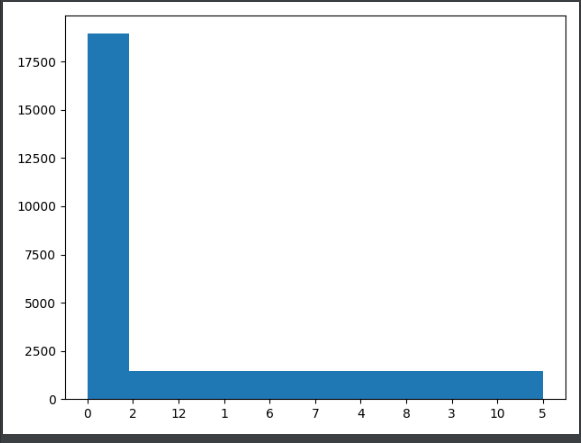
\includegraphics[scale=0.45]{zero-values-votes.png}
\caption{Prikaz porazdelitve točk vseh glasov med letoma 1975 in 2019.}
\label{slika1}
\end{center}
\end{figure}

Zanima nas, kako so te točke porazdeljene. Pomagal sem si s funkcijo za izris histograma hist() iz knjižnice matplotlib.
Opazimo lahko, da je glasov z vrednostjo 0 občutno več, kot vseh ostalih. To je precej pričakovano, saj je na enem dogodku
tekmovalo tudi do 53 držav, točke (x $>$ 0) pa lahko dodeliš le 12 državam. Zato kar nekaj (večina) polj s točkami vsebuje vrednost 0.
Po podrobnejšem pregledu ostalih vrednosti se lepo vidi tudi, da je ostalih točk enako.
\\Tudi to je precej samoumevno -
glasove vedno oddaš za vse možne točke (ne moreš se vzdržati na primer glasu za maksimalno število točk...).

Za lažjo analizo podatkov sem iz slovarja izločil vse države, ki so se na tekmovanju pojavile 5x ali manj. V tem primeru so bile
to Moroko, Srbija in črna gora, Avstralija in Severna Makedonija. Slednja se je na tekmovanju pojavila samo enkrat, kar se
mi ni zdelo smiselno oziroma omembe vredno. Zanimajo nas bolj "stare članice".

\section{Računanje razdalj.}
Pri gručenju držav, ki se med seboj favorizirajo, sem za njihovo podobnost glasovanja uporabil evklidsko razdaljo.
Bistvene razlike med evklidsko in manhattansko razdaljo nisem opazil. Menim, da bi bile obe dovolj dobri.
Pri računanju razdalje med dvema clusterjema sem se sprehodil čez vse možne kombinacije pripadnikov teh dveh gruč.
To je sicer kar potratno, kar se tiče časovne kompleksnosti, o čimer bom več povedal na koncu.

Ko so posamezne gruče vsebovale po več držav, sem za izračun razdalje med gručami uporabljal povprečno razdaljo
(\href{https://www.statistics.com/glossary/average-linkage-clustering/}{average linkage}).
\\Države gruč z najmanjšo razdaljo so bile združene v eno gručo. Ta postopek je potekal vse dokler nismo imeli le še ene
gruče z vsemi državami.

Tu lako vidimo osrčje računanja povprečne dolžine med dvema skupinama držav. Algoritem se sprehodi skozi vse države znotraj
obeh skupin in jih "primerja" med seboj. Primerja jih na način da kliče funkcijo row\_distance(), ki kot argument sprejme
imeni dveh držav in vrne evklidsko razdaljo njunih vektorjev glasovanja.

\begin{lstlisting}[language=Python, caption=merge\_clusters(clusters{,} c1{,} c2)]
for c in c1_flat:
    for d in c2_flat:
        # distance between c & d
        dist += self.row_distance(c[0], d[0])
dist /= (len(c1_flat) * len(c2_flat))
\end{lstlisting}

Računanje \href{https://en.wikipedia.org/wiki/Euclidean_distance}{evklidske razdalje} dveh vektorjev p in q:

\begin{lstlisting}[language=Python, caption=euclidean distance]
e = sum((p - q) ** 2 for p, q in zip(v1, v2)) ** .5
\end{lstlisting}

Končen ASCII izris dendrograma sem implementiral z rekurzivno funkcijo, ki kot argument prejme en objekt tipa list.
List vsebuje eno skupino (vseh) držav, ki se nato razdeli na dve podskupini, vsaka izmed njih še na dve in tako naprej
vse dokler ne dobimo posameznih držav.
\pagebreak
\begin{lstlisting}[language=Python, caption=Function izris()]
def izris(arr, i):
    if len(arr) == 1:
        print("    " * i, "---- ", arr[0], sep='')
    else:
        i += 1
        izris(arr[0], i)
        print("    " * (i - 1), "----|", sep='')
        izris(arr[1], i)
\end{lstlisting}

\begin{figure}[h!]
\begin{center}
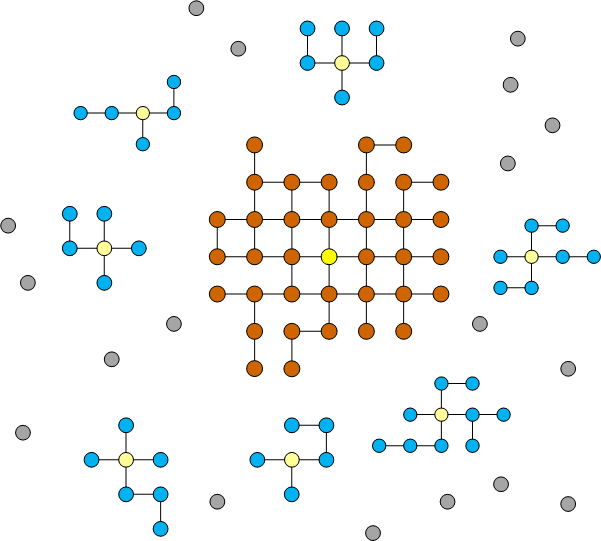
\includegraphics[scale=03]{slika-primer.png}
\caption{Vsako sliko opremi s podnapisom, ki pove, kaj slika prikazuje.}
\label{slika2}
\end{center}
\end{figure}

\section{Dendrogram.} $\downarrow$
\begin{lstlisting}
        ---- Greece
    ----|
        ---- Cyprus
----|
                ---- Malta
            ----|
                    ---- Turkey
                ----|
                        ---- Luxembourg
                    ----|
                        ---- Italy
        ----|
                        ---- Lithuania
                    ----|
                        ---- Latvia
                ----|
                    ---- Estonia
            ----|
                            ---- Slovenia
                        ----|
                                ---- F.Y.R. Macedonia
                            ----|
                                    ---- Croatia
                                ----|
                                    ---- Bosnia & Herzegovina
                    ----|
                        ---- Albania
                ----|
                            ---- Romania
                        ----|
                            ---- Moldova
                    ----|
                            ---- Poland
                        ----|
                                    ---- Montenegro
                                ----|
                                                ---- San Marino
                                            ----|
                                                    ---- Hungary
                                                ----|
                                                        ---- Serbia
                                                    ----|
                                                        ---- Czech Republic
                                        ----|
                                            ---- Bulgaria
                                    ----|
                                            ---- Yugoslavia
                                        ----|
                                                    ---- Slovakia
                                                ----|
                                                    ---- Monaco
                                            ----|
                                                ---- Andorra
                            ----|
                                        ---- Belarus
                                    ----|
                                            ---- Georgia
                                        ----|
                                                ---- Russia
                                            ----|
                                                    ---- Ukraine
                                                ----|
                                                    ---- Azerbaijan
                                ----|
                                    ---- Armenia
    ----|
                        ---- Israel
                    ----|
                                ---- United Kingdom
                            ----|
                                ---- Ireland
                        ----|
                                ---- Switzerland
                            ----|
                                        ---- Germany
                                    ----|
                                            ---- The Netherlands
                                        ----|
                                            ---- Belgium
                                ----|
                                    ---- Austria
                ----|
                            ---- Spain
                        ----|
                            ---- Portugal
                    ----|
                        ---- France
            ----|
                ---- Finland
        ----|
                ---- Iceland
            ----|
                        ---- Sweden
                    ----|
                        ---- Norway
                ----|
                    ---- Denmark
\end{lstlisting}

\begin{figure}[h!]
\begin{center}
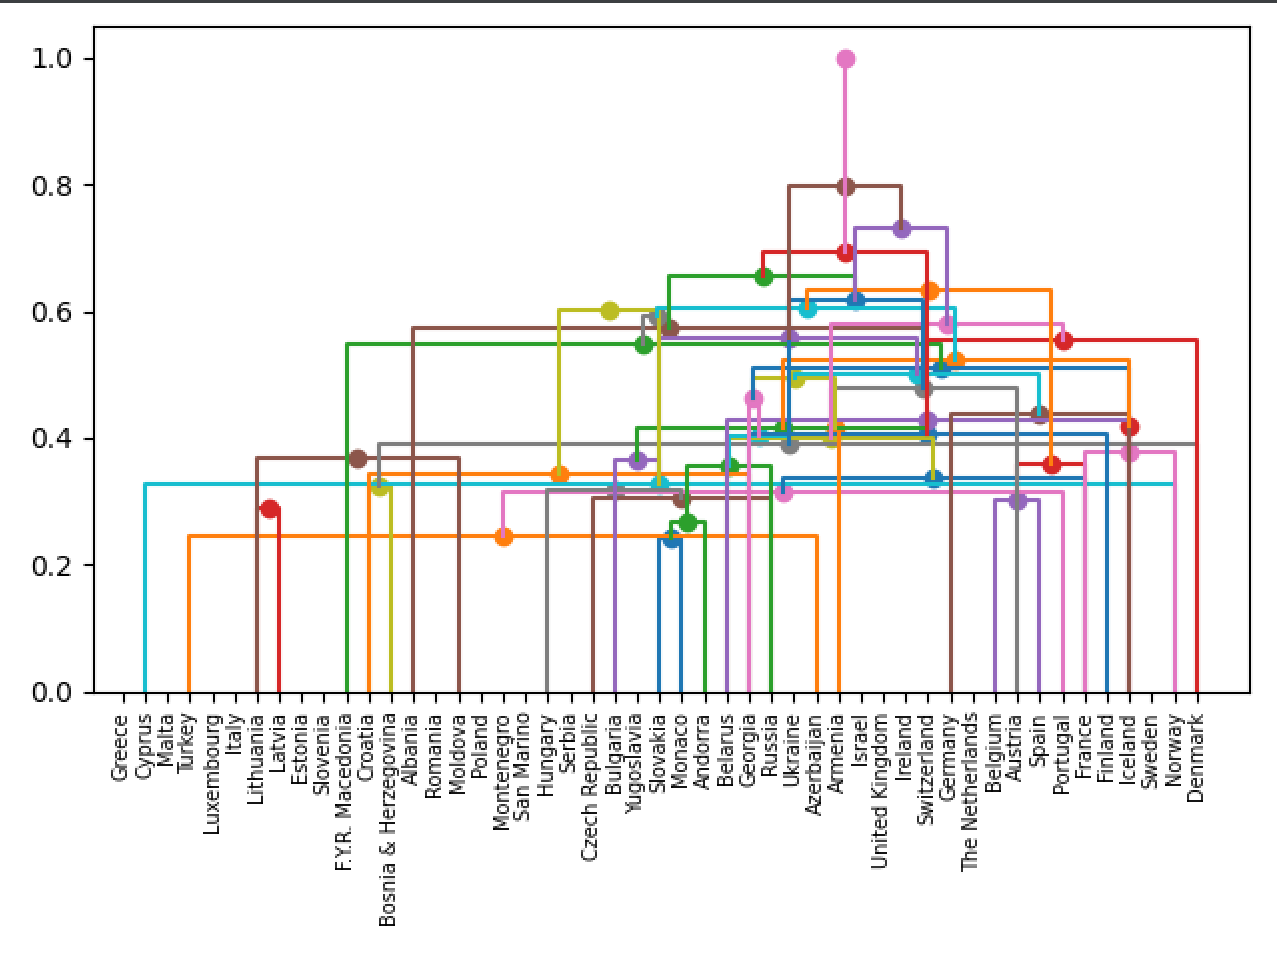
\includegraphics[scale=0.45]{graphical.png}
\caption{Grafični prikaz ASCII dendrograma (z ustreznimi normaliziranimi dolžinami) zgoraj.}
\label{slika3}
\end{center}
\end{figure}


\section{Skupine in njihove preferenčne izbire.}
%%%%%%%%%%%%%%%%%%%%%%%%%%%%%%%%%%%%%%%%%%%%%%%%%%%%%%%%%%%%%%%%%%%%%%%%%%%%%%%%%%%%%%%%%%%%%%%%
Skupine in njihove preferenčne izbire. Glede na rezultate razvrščanja smiselno določite skupine. Vsaki skupini v tabeli dopišite preferirane države in tiste, za katere ne glasujejo. Opišite, kako ste določili skupine in preferirane države. (1 tabela in 1 odstavek)

\begin{table}[htbp]
\caption{Preferenčne skupine držav in njihove članice}
\label{tab1}
\begin{center}
\begin{tabular}{llp{3cm}}
\hline
ime spremenljivke & definicijsko območje & opis \\
\hline
cena & [0, 500] & cena izdelka v EUR\\
teža & [1, 1000] & teža izdelka v dag \\
kakovost & [slaba|srednja|dobra] & kakovost izdelka \\
\hline
\end{tabular}
\end{center}
\end{table}



%%%%%%%%%%%%%%%%%%%%%%%%%%%%%%%%%%%%%%%%%%%%%%%%%%%%%%%%%%%%%%%%%%%%%%%%%%%%%%%%%%%%%%%%%%%%%%%%

V tem poglavju podaš rezultate s kratkim (enoodstavčnim)
komentarjem. Rezultate lahko prikažeš tudi v tabeli (primer je
tabela~\ref{tab1}).

Odstavke pri pisanju poročila v LaTeX-u ločiš tako, da pred novim
odstavkom pustiš prazno vrstico. Tudi, če pišeš poročilo v kakšnem
drugem urejevalniku, morajo odstavki biti vidno ločeni. To narediš z
zamikanjem ali pa z dodatnim presledkom.

\begin{table}[htbp]
\caption{Atributi in njihove zaloge vrednosti.}
\label{tab1}
\begin{center}
\begin{tabular}{llp{3cm}}
\hline
ime spremenljivke & definicijsko območje & opis \\
\hline
cena & [0, 500] & cena izdelka v EUR\\
teža & [1, 1000] & teža izdelka v dag \\
kakovost & [slaba|srednja|dobra] & kakovost izdelka \\
\hline
\end{tabular}
\end{center}
\end{table}

Podajanje rezultati naj bo primerno strukturirano. Če ima naloga več
podnalog, uporabi podpoglavja. Če bi želel poročati o rezultatih
izčrpno in pri tem uporabiti vrsto tabel ali grafov, razmisli o
varianti, kjer v tem poglavju prikažeš in komentiraš samo glavne
rezultate, kakšne manj zanimive detajle pa vključite v prilogo (glej
prilogi~\ref{app-res} in~\ref{app-code}).

\section{Izjava o izdelavi domače naloge.}
Domačo nalogo in pripadajoče programe sem izdelal sam.

\appendix
\appendixpage
\section{\label{app-res}Podrobni rezultati poskusov.}

Če je rezultatov v smislu tabel ali pa grafov v nalogi mnogo,
predstavi v osnovnem besedilu samo glavne, podroben prikaz
rezultatov pa lahko predstaviš v prilogi. V glavnem besedilu ne
pozabi navesti, da so podrobni rezultati podani v prilogi.

\section{\label{app-code}Programska koda.}

Za domače naloge bo tipično potrebno kaj sprogramirati. Če ne bo od
vas zahtevano, da kodo oddate posebej, to vključite v prilogo. Čisto
za okus sem tu postavil nekaj kode, ki uporablja Orange
(\url{http://www.biolab.si/orange}) in razvrščanje v skupine.


\begin{lstlisting}
import random
import Orange

data_names = ["iris", "housing", "vehicle"]
data_sets = [Orange.data.Table(name) for name in data_names]

print "%10s %3s %3s %3s" % ("", "Rnd", "Div", "HC")
for data, name in zip(data_sets, data_names):
    random.seed(42)
    km_random = Orange.clustering.kmeans.Clustering(data, centroids = 3)
    km_diversity = Orange.clustering.kmeans.Clustering(data, centroids = 3,
        initialization=Orange.clustering.kmeans.init_diversity)
    km_hc = Orange.clustering.kmeans.Clustering(data, centroids = 3,
        initialization=Orange.clustering.kmeans.init_hclustering(n=100))
    print "%10s %3d %3d %3d" % (name, km_random.iteration, \
    km_diversity.iteration, km_hc.iteration)
\end{lstlisting}

\end{document}
